%!TEX program = pdflatex
\documentclass[10pt]{article}
\usepackage[pdftex]{graphicx, color}
\usepackage{listings}
\usepackage{graphicx}
\usepackage{mathtools}
\usepackage{tikz}
\usetikzlibrary{automata,positioning}

\headheight 8pt \headsep 20pt \footskip 30pt
\textheight 9in \textwidth 6.5in
\oddsidemargin 0in \evensidemargin 0in
\topmargin -.35in

\lstset{basicstyle=\small\ttfamily,breaklines=true}
\newcommand {\pts}[1]{{\bf #1 pts}}
\newcommand{\ttmath}[1]{$\mathtt{#1}$} 
\newcommand{\ossimple}[6]{#1,#2,#3\vdash #4 : #5,#6}
\newcommand{\osrule}[8]{\frac{#7}{\ossimple{#1}{#2}{#3}{#4}{#5}{#6}}\eqno
  \mbox{#8}}
  
\begin{document}
\begin{center}
\Large CS131 Compilers: Writing Assignment 4\\Due Saturday, June 12, 2021 at 23:59pm
\end{center}

\begin{center}
%% Change this:
\LARGE Name - Numbber
\end{center}

This assignment asks you to prepare written answers to questions on
run-time environment, object layout, operational semantics, code generation, register allocation and garbage collection.
Each of the questions has a short answer. You
may discuss this assignment with other students and work on the problems
together. However, your write-up should be your own individual work.
and you should indicate in your submission who you worked with, if applicable.
Written assignments are turned in at the start of lecture.
You should use the Latex template provided at the course web site to write your solution.

\begin{center}
%% Change this:
I worked with: ()()
\end{center}

Example for operational semantics rule in tex:
$$\osrule{so}{S_1} E {\mbox{while }e_1\mbox{ loop } e_2\mbox{ pool}}{void}{S_{2}}
	{\begin{array}{l}
	\ossimple{so}{S_1}{E}{e_1}{Bool(false)}{S_2}\\
	 \end{array}}{[Loop-False]}
$$

\begin{enumerate}

\item (10 pts)
Consider the following Cool classes:

\begin{center}
\begin{minipage}{6cm}
\begin{verbatim}
class A {
    a1 : Int;
    a2 : String;
    m1() : Object { ... };
    m2() : Object { ... };
};

class B inherits A {
    a3 : Int;
    m1() : Object { ... };
    m3() : Object { ... };
};

class C inherits B {
    a4 : Int;
    m2() : Object { ... };
    m3() : Object { ... };
};
\end{verbatim}
\end{minipage}
\end{center}
\begin{enumerate}

\item Draw a diagram that illustrates the layout of objects of type {\tt
A}, {\tt B} and {\tt C}, including their dispatch tables.
\begin{table}[h]
  \centering
  \begin{tabular}{llll|l|}
  \cline{1-1} \cline{3-3} \cline{5-5}
  \multicolumn{1}{|l|}{0: A Tag}  & \multicolumn{1}{l|}{} & \multicolumn{1}{l|}{0: B Tag}  &  & 0: C Tag  \\ \cline{1-1} \cline{3-3} \cline{5-5} 
  \multicolumn{1}{|l|}{4: 5}      & \multicolumn{1}{l|}{} & \multicolumn{1}{l|}{4: 6}      &  & 4: 7      \\ \cline{1-1} \cline{3-3} \cline{5-5} 
  \multicolumn{1}{|l|}{8: *}      & \multicolumn{1}{l|}{} & \multicolumn{1}{l|}{8: *}      &  & 8: *      \\ \cline{1-1} \cline{3-3} \cline{5-5} 
  \multicolumn{1}{|l|}{12: $a_1$} & \multicolumn{1}{l|}{} & \multicolumn{1}{l|}{12: $a_1$} &  & 12: $a_1$ \\ \cline{1-1} \cline{3-3} \cline{5-5} 
  \multicolumn{1}{|l|}{16: $a_2$} & \multicolumn{1}{l|}{} & \multicolumn{1}{l|}{16: $a_2$} &  & 12: $a_2$ \\ \cline{1-1} \cline{3-3} \cline{5-5} 
                                  & \multicolumn{1}{l|}{} & \multicolumn{1}{l|}{20: $a_3$} &  & 20: $a_3$ \\ \cline{3-3} \cline{5-5} 
                                  &                       &                                &  & 24: $a_4$ \\ \cline{5-5} 
  \end{tabular}
  \end{table}
  \begin{table}[h]
    \centering
    \begin{tabular}{lllllll}
    \cline{1-1} \cline{3-3} \cline{5-5}
    \multicolumn{1}{|l|}{A}                    & \multicolumn{1}{l|}{} & \multicolumn{1}{l|}{B}                    & \multicolumn{1}{l|}{} & \multicolumn{1}{l|}{C}                    &  &  \\ \cline{1-1} \cline{3-3} \cline{5-5}
    \multicolumn{1}{|l|}{0: Object.abort}      & \multicolumn{1}{l|}{} & \multicolumn{1}{l|}{0: Object.abort}      & \multicolumn{1}{l|}{} & \multicolumn{1}{l|}{0: Object.abort}      &  &  \\ \cline{1-1} \cline{3-3} \cline{5-5}
    \multicolumn{1}{|l|}{4: Object.type\_name} & \multicolumn{1}{l|}{} & \multicolumn{1}{l|}{4: Object.type\_name} & \multicolumn{1}{l|}{} & \multicolumn{1}{l|}{4: Object.type\_name} &  &  \\ \cline{1-1} \cline{3-3} \cline{5-5}
    \multicolumn{1}{|l|}{8: Object.copy}       & \multicolumn{1}{l|}{} & \multicolumn{1}{l|}{8: Object.copy}       & \multicolumn{1}{l|}{} & \multicolumn{1}{l|}{8: Object.copy}       &  &  \\ \cline{1-1} \cline{3-3} \cline{5-5}
    \multicolumn{1}{|l|}{12: A.m1}             & \multicolumn{1}{l|}{} & \multicolumn{1}{l|}{12: B.m1}             & \multicolumn{1}{l|}{} & \multicolumn{1}{l|}{12: A.m1}             &  &  \\ \cline{1-1} \cline{3-3} \cline{5-5}
    \multicolumn{1}{|l|}{16: A.m2}             & \multicolumn{1}{l|}{} & \multicolumn{1}{l|}{16: A.m2}             & \multicolumn{1}{l|}{} & \multicolumn{1}{l|}{16: C.m2}             &  &  \\ \cline{1-1} \cline{3-3} \cline{5-5}
                                               & \multicolumn{1}{l|}{} & \multicolumn{1}{l|}{20: B.m3}             & \multicolumn{1}{l|}{} & \multicolumn{1}{l|}{20: C.m3}             &  &  \\ \cline{3-3} \cline{5-5}
                                               &                       &                                           &                       &                                           &  & 
    \end{tabular}
    \end{table}
    \newpage
\item Let {\tt obj} be a variable whose static type is {\tt A}.  Assume
that {\tt obj} is stored in register {\tt \$a0}.  Write MIPS code for the
function invocation {\tt obj.2()}.  You may use temporary registers
such as {\tt \$t0} if you wish.
\begin{verbatim}
  lw     $t0, 8($a0)
  lw     $t1, 16($t0)             
  jalr   $t1                           
\end{verbatim}
\item Explain what happens in part (b) if {\tt obj} has dynamic type {\tt
B}.

It will invoke correctly. We can visit the type's objects throuth the dispatch pointer at the offset 8. (b) and (c) will all visit A.m2 since B inherits from A and do not override A.m2.

\end{enumerate}

\medskip

\item (10 pts)
Suppose you wish to add arrays to Cool using the following syntax:

\begin{center}
\begin{tabular}{ll}
\texttt{let a:T[\ttmath{e_1}] in \ttmath{e_2}} &
  Create an array $a$ with size $e_1$ of $T$'s, usable in $e_2$ \\
\texttt{a[\ttmath{e_1}] <- \ttmath{e_2}} &
  Assign $e_2$ to element $e_1$ in $a$ \\
\texttt{a[e]} &
  Get element $e$ of $a$
\end{tabular}
\end{center}

Write the operational semantics for these three syntactic constructs. You
may find it helpful to think of an array of type $T[n]$ as an object with
$n$ attributes of type $T$.
$$
\osrule{so}{S_1}{E_1}{\mbox{let } a:T[e_1] \mbox{ in } e_2}{v_2}{S_{4}}
	{\begin{array}{l}
	\ossimple{so}{S_1}{E_1}{e_1}{\mbox{Int}(n)}{S_2}\\
	l_i = \mbox{newloc}(S_2) \mbox{ for } i = 0 \dots n \mbox{ and each } l_i \mbox{ is distinct }\\
	v_a = \mbox{array}(a_1:l_1, \dots, a_n:l_n)\\
	S_3 = S_2[v_a/l_0, D_T/l_1, \dots, D_T/l_n]\\
	E_2 = E_1[l_0/a]\\
	\ossimple{so}{S_3}{E_2}{e_2}{v_2}{S_4}
	 \end{array}}{}
$$

$$
\osrule{so}{S_1}{E}{a[e_1] \mbox{\texttt{ <- }} e_2}{v_2}{S_{4}}
	{\begin{array}{l}
	\ossimple{so}{S_1}{E}{e_1}{\mbox{Int}(m)}{S_2}\\
	\ossimple{so}{S_2}{E}{e_2}{v_2}{S_3}\\
	E(a) = l_a\\
	S_2(l_a) = \mbox{array}(a_1:l_1, \dots, a_n:l_n)\\
	1 \le m \le n\\
	S_4 = S_3[v_2/l_m]
	 \end{array}}{}
$$

$$
\osrule{so}{S_1}{E}{a[e]}{v}{S_2}
	{\begin{array}{l}
	\ossimple{so}{S_1}{E}{e_1}{\mbox{Int}(m)}{S_2}\\
	E(a) = l_a\\
	S_2(l_a) = \mbox{array}(a_1:l_1, \dots, a_n:l_n)\\
	1 \le m \le n\\
	v = S_2(l_m)
	 \end{array}}{}
$$
\pagebreak

\item (10 pts)
The operational semantics for Cool's {\tt while} expression show that
result of evaluating such an expression is always {\tt void}.  (See page
28 of the Cool manual.)

However, we could have used the following alternative semantics:

\begin{itemize}

\item If the loop body executes at least once, the result of the {\tt
while} expression is the result from the last iteration of the loop body.

\item If the loop body never executes (i.e., the condition is false the
first time it is evaluated), then the result of the {\tt while} expression
is {\tt void}.

\end{itemize}

For example, consider the following expression:

\begin{center}
{\tt while (x < 10) loop x <- x+1 pool}
\end{center}

The result of this expression would be 10 if {\tt x} $<$ 10 or {\tt void}
if {\tt x} $\geq$ 10.

Write new operational rules for the {\tt while} construct that formalize
these alternative semantics.


$$
\osrule{so}{S_1} E {\mbox{while }e_1\mbox{ loop } e_2\mbox{ pool}}{void}{S_{2}}
	{\begin{array}{l}
	\ossimple{so}{S_1}{E}{e_1}{Bool(false)}{S_2}\\
	 \end{array}}{[Loop-False]}
$$

$$
\osrule{so}{S_1} E {\mbox{while }e_1\mbox{ loop } e_2\mbox{ pool}}{v_2}{S_{4}}
	{\begin{array}{l}
	\ossimple{so}{S_1}{E}{e_1}{Bool(true)}{S_2}\\
	\ossimple{so}{S_2}{E}{e_2}{v_2}{S_3}\\
	\ossimple{so}{S_3}{E}{e_1}{Bool(false)}{S_4}\\
	 \end{array}}{[Loop-True-Last]}
$$

$$
\osrule{so}{S_1} E {\mbox{while }e_1\mbox{ loop } e_2\mbox{ pool}}{v_3}{S_{5}}
	{\begin{array}{l}
	\ossimple{so}{S_1}{E}{e_1}{Bool(true)}{S_2}\\
	\ossimple{so}{S_2}{E}{e_2}{v_2}{S_3}\\
	\ossimple{so}{S_3}{E}{e_1}{Bool(true)}{S_4}\\
	\ossimple{so}{S_3}{E}{\mbox{while }e_1\mbox{ loop } e_2\mbox{ pool}}{v_3}{S_5}\\
	 \end{array}}{[Loop-True-Not-Last]}
$$

\item (10 pts) Consider the following MIPS assembly code program.  Using the
stack-machine based code generation rules from lecture, what source program produces this
code?
\begin{verbatim}
f_entry(int):
  addiu   $sp,$sp,-32
  sw      $31,28($sp)
  sw      $fp,24($sp)
  move    $fp,$sp
  sw      $4,32($fp)
  lw      $2,32($fp)
  slt     $2,$2,2
  beq     $2,$0,body
  li      $2,1                 
  b       end

body:
  lw      $2,32($fp)
  addiu   $2,$2,-1
  move    $4,$2
  jal     f_entry(int)
  move    $3,$2
  lw      $2,32($fp)
  mult    $3,$2
  mflo    $2
end:
  move    $sp,$fp
  lw      $31,28($sp)
  lw      $fp,24($sp)
  addiu   $sp,$sp,32
  j       $31
\end{verbatim}
\begin{verbatim}
int f(int x){
  if (x < 2){
    return 1;
  }
  else{
    return x*f(x-1);
  }
}
\end{verbatim}


\item (10 pts) Consider the following code in python dialect, The following steps are dependent, do the optimization until un-optimizable.
\begin{verbatim}
  p = 3
  r = 10
  s = p + r
  t = 2*r + s
  t = p
  u = p + r
  v = p + t
  y[1] = 3
  y[2] = 3
  y[3] = 3
  y[4] = 3
  for i in range(1,4):
    y[i] + v
  w = 3 + x
\end{verbatim}
\begin{enumerate}
  \item Do Dead Code Elimination.
  \item Do Common Subexpression Elimination.
  \item Do Copy Propagation
  \item Do Constant Folding and Constant Propagation
  \item Do Vectorization
\end{enumerate}

\newpage
(a)\\
$-$ t = 2*r + s\\
$-$ for i in range(1,4): \\
$-$ y[i] + v\\
(b)\\
$-$  u = p + r \\
$+$  u = s \\
(c) \\
$-$  s = p + r \\
$+$  s = 3 + 10 \\
$-$ t = p \\
$+$ t = 3\\
$-$  v = p + t \\
$+$  v = 3 + 3 \\
(d) \\
$- $s = 3 + 10  \\
$+$ s = 13\\
$-$ v = 3 + 3 \\
$+$ v = 6 \\
(e)\\
$-$y[1] = 3\\
$-$y[2] = 3\\
$-$y[3] = 3\\
$-$y[4] = 3\\
$+$
\{y[0], y[1], y[2], y[3]\} = \{3,3,3,3\} \\
(c) \\
$-$  u = s \\
$+$ u = 13 \\
\textbf{Result:} 
\begin{verbatim}
  p = 3
  r = 10
  s = 13 
  t = 3
  u = 13
  v = 6
  {y[0], y[1], y[2], y[3]} = {3,3,3,3}
  w = 3 + x
\end{verbatim}



\item (2*10=20 pts) Consider the following program:

\begin{verbatim}
L0: e := 0
    b := 1;
    d := 2;
    c := 4;
L1: a := b+2
    e := e + c
    f := a * a
    if f < c goto L3
L2: e := e + f
    c := d + 5
    goto L4
L3: d := d + 4
    b := b - 4
    if b != d goto L1
    goto L3
L4:
\end{verbatim}

This program uses six temporaries \texttt{a}-\texttt{f}.  Assume that
our machine has only 4 available registers \texttt{\$r0},
\texttt{\$r1}, \texttt{\$r2}, and \texttt{\$r3}
and that only
\texttt{e} is live on exit from this program.

\begin{enumerate}
\item Compute the Calculate live-in and live-out at each statement and drzaw the register interference graph.  (Computing the sets of
live variables at every program point may be helpful for this step.)


\[
  %% Your answer here
  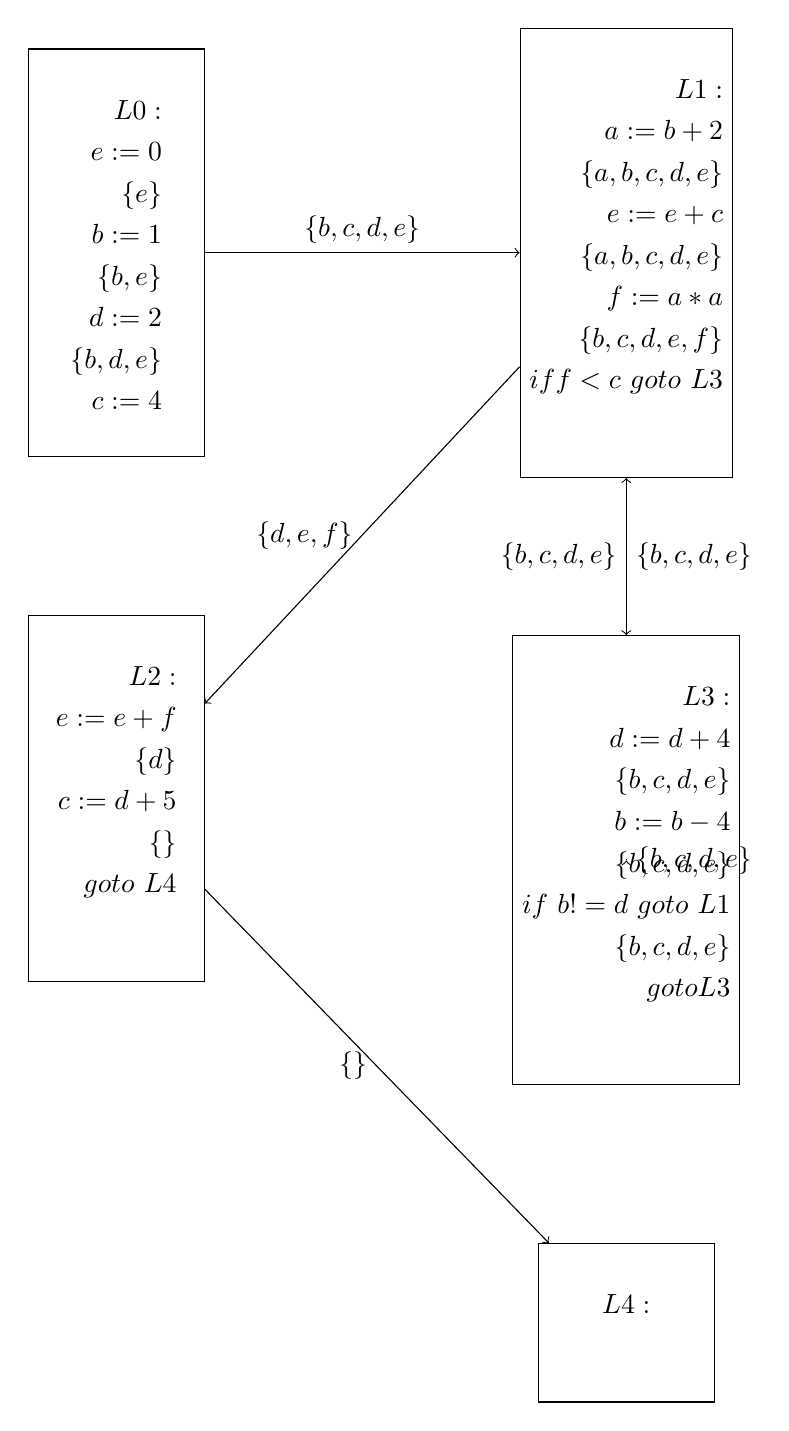
\begin{tikzpicture}[node distance=2cm and 4cm] 
      \node[rectangle, draw = black] (0) {
          \parbox{2cm}{
              \begin{align*}
                L0: \\
                e := 0 \\
                \{ e\} \\
                b := 1 \\
                \{ b,e \} \\
                d := 2 \\
                \{  b,d,e\} \\
                c := 4
              \end{align*}
          }
      };
      \node[rectangle, draw = black,right = of 0] (1) {
        \parbox{2cm}{
            \begin{align*}
              L1: \\
              a := b + 2 \\
              \{ a,b,c,d,e \} \\
              e:= e + c \\
              \{ a,b,c,d,e\} \\
              f := a * a \\
              \{ b,c,d,e,f\} \\
              if f < c ~ goto ~L3 \\
            \end{align*}
        }
    };

    \node[rectangle, draw = black,below = of 0] (2) {
        \parbox{2cm}{
            \begin{align*}
              L2: \\
              e := e + f\\
              \{ d \}\\
              c := d + 5\\
              \{ \} \\
              goto ~L4\\
            \end{align*}
        }
    };

    \node[rectangle, draw = black,below = of 1] (3) {
      \parbox{2cm}{
          \begin{align*}
            L3: \\
            d := d + 4\\
            \{  b,c,d,e \} \\
    b := b - 4\\
    \{  b,c,d,e\} \\
    if ~b != d ~goto~ L1\\
    \{  b,c,d,e \} \\
    goto L3\\
          \end{align*}
      }
  };

  \node[rectangle, draw = black,below = of 3] (4) {
    \parbox{2cm}{
        \begin{align*}
          L4: \\
        \end{align*}
    }
};
    \path[->]
    (0) 	edge 		node[above]{$ \{ b,c,d,e\} $} (1)
    (1) 	edge 		node[left]{$ \{ d,e,f \} $} (2)
    (1) 	edge 		node[ left]{$ \{  b,c,d,e \} $} (3)
    (3) 	edge 		node[ right]{$ \{  b,c,d,e\} $} (1)
    (3) 	edge 		node[loop right]{$ \{  b,c,d,e \} $} (3)
    (2) 	edge 		node[left]{$ \{  \} $} (4);
\end{tikzpicture}
  \]\\\\\\
  \begin{center}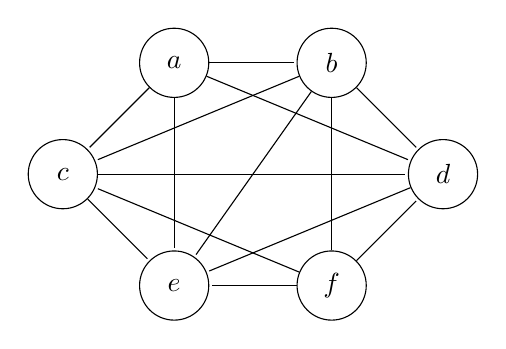
\begin{tikzpicture}[shorten >=1pt,node distance=2cm,on grid,auto]
      \node[state] 	(c) 						{$c$};
      \node[state] 	(a) 	[above right=of c]	{$a$};
      \node[state]	(e) 	[below right=of c] 	{$e$};
      \node[state] 	(b) 	[	   right=of a] 	{$b$};
      \node[state] 	(d) 	[below right=of b] 	{$d$};
      \node[state] 	(f) 	[	   right=of e]	{$f$};
      \path[-]
      (a) 	edge	node	{} 		(b)
          edge	node	{} 		(c)
          edge	node	{} 		(d)
          edge	node	{} 		(e)
      (b) 	edge	node	{} 		(c)
          edge	node	{} 		(d)
          edge	node	{} 		(e)
          edge	node	{} 		(f)
      (c)		edge	node	{} 		(d)
          edge	node	{} 		(e)
       
      (d) 	edge	node	{} 		(e)
      (f) 	edge	node	{} 		(b)
      	edge	node	{} 		(c)
      	edge	node	{} 		(d)
        edge	node	{} 		(e)
      ;
     
    \end{tikzpicture}\end{center}

\item Use the graph coloring heuristics discussed in lecture to assign
  each temporary to a register on a machine that has $4$ registers.
Rewrite the program replacing temporaries by registers and including whatever
spill code is necessary.  Use the pseudo-instructions \texttt{load x}
and \texttt{store x} to load and spill the value of \texttt{x} from
memory.
\end{enumerate}
\begin{enumerate}
\item pick b as a candidate for spilling 
\begin{center}\begin{tikzpicture}[shorten >=1pt,node distance=2cm,on grid,auto]
  \node[state] 	(c) 						{$c$};
  \node[state] 	(a) 	[above right=of c]	{$a$};
  \node[state]	(e) 	[below right=of c] 	{$e$};
  \node[state] 	(d) 	[below right=of b] 	{$d$};
  \node[state] 	(f) 	[	   right=of e]	{$f$};
  \path[-]
  (a) 	
      edge	node	{} 		(c)
      edge	node	{} 		(d)
      edge	node	{} 		(e)

  (c)		edge	node	{} 		(d)
      edge	node	{} 		(e)
   
  (d) 	edge	node	{} 		(e)
  (f) 	
    edge	node	{} 		(c)
    edge	node	{} 		(d)
    edge	node	{} 		(e)
  ;
 
\end{tikzpicture}\end{center}

\item  remove a, stack:a 
\begin{center}\begin{tikzpicture}[shorten >=1pt,node distance=2cm,on grid,auto]
  \node[state] 	(c) 						{$c$};
  \node[state]	(e) 	[below right=of c] 	{$e$};
  \node[state] 	(d) 	[below right=of b] 	{$d$};
  \node[state] 	(f) 	[	   right=of e]	{$f$};
  \path[-]
  (c)		edge	node	{} 		(d)
      edge	node	{} 		(e)
   
  (d) 	edge	node	{} 		(e)
  (f) 	
    edge	node	{} 		(c)
    edge	node	{} 		(d)
    edge	node	{} 		(e)
  ;
 
\end{tikzpicture}\end{center}
\item  remove f, stack:a,f 
\begin{center}\begin{tikzpicture}[shorten >=1pt,node distance=2cm,on grid,auto]
  \node[state] 	(c) 						{$c$};
  \node[state]	(e) 	[below right=of c] 	{$e$};
  \node[state] 	(d) 	[below right=of b] 	{$d$};
  \path[-]
  (c)		edge	node	{} 		(d)
      edge	node	{} 		(e)
  (d) 	edge	node	{} 		(e)
  ;
 
\end{tikzpicture}\end{center}

\item  remove c, stack:a,f,c
\begin{center}\begin{tikzpicture}[shorten >=1pt,node distance=2cm,on grid,auto]
  \node[state]	(e) 	[below right=of c] 	{$e$};
  \node[state] 	(d) 	[below right=of b] 	{$d$};
  \path[-]
  (d) 	edge	node	{} 		(e)
  ;
 
\end{tikzpicture}\end{center}

\item remove e,d, stack:a,f,c,e,d

\end{enumerate}
The result is \\
e: \$r0 \\
d: \$r1 \\
c: \$r2 \\
f: \$r3 \\
a: \$r3 \\
b: in Memory

\begin{verbatim}
L0: 
    $r0 := 0;
    $r3 := 1;
    store $r3
   
    $r1 = 2;
    $r2 := 4;
L1: 
    load $r3
    $r3 := $r3+2
    $r0 := $r0 + $r2
    $r3 := $r3 * $r3
    if $r3 < $r2 goto L3
L2: $r0 := $r0 + $r3
    $r2 := $r1 + 5
    goto L4
L3: $r1 := $r1 + 4
    load $r3
    $r3 := $r3 - 4
    if $r3!= $r1 goto L1
    goto L3
L4:
\end{verbatim}


\item (10*3=30 pts) Consider the following Cool program:

\begin{verbatim}
class C {
  x : C; y : C;
  setx(newx : C) : C { x <- newx };
  sety(newy : C) : C { y <- newy };
  setxy(newx : C, newy :C) : SELF_TYPE {{ x <- newx; y <- newy; self; }};
};

class Main {
  x:C;
  main() : Object {
    let a : C <- new C, b :C <- new C, c : C<- new C, d : C <- new C,
    e : C <- new C, f :C <- new C, g : C <- new C, h : C <- new C in {
      f.sety(a), a.setxy(e, c); b.setx(d); g.setxy(d,f); c.sety(h); h.setxy(e, g); x <- c;
    }
  };
};
\end{verbatim}
\begin{enumerate}
  \item (10 pts) Draw the heap at the end of execution of the above program, identifying objects by the variable names to which they are bound in the let expression. Assume that the root is the Main object created at the start of the program, and this object is not in the heap (note that Main is pointing to c).
%



\begin{center}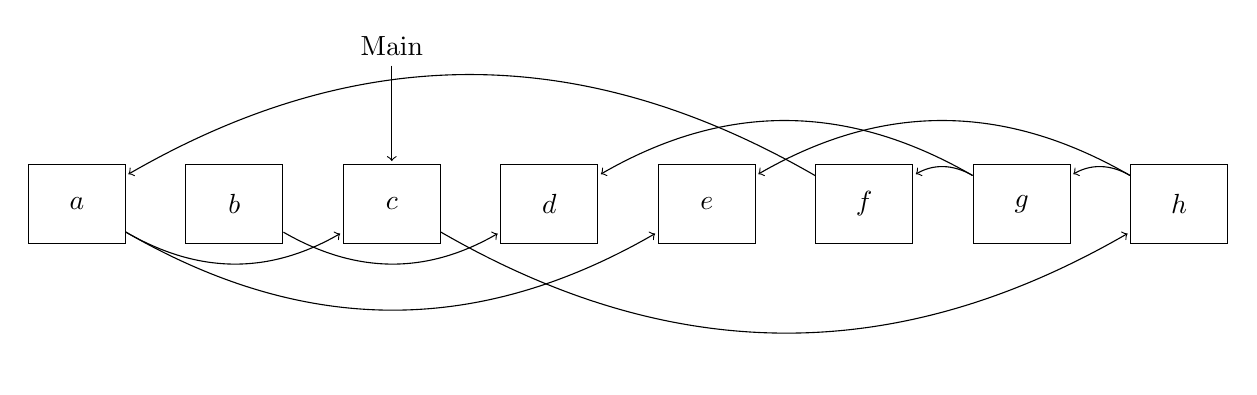
\begin{tikzpicture}[shorten >=1pt,node distance=2cm,on grid,auto]
  \tikzset{
    rect1/.style = {
      shape = rectangle,
      draw = black,
      text width = 1cm,
      align = center,
      minimum height = 1cm,
    }
  }
  \node[rect1] 			(a) 					{$a$};
  \node[rect1] 			(b) 	[right=of a]	{$b$};
  \node[rect1]			(c) 	[right=of b] 	{$c$};
  \node[rect1] 			(d) 	[right=of c] 	{$d$};
  \node[rect1] 			(e) 	[right=of d] 	{$e$};
  \node[rect1] 			(f) 	[right=of e]	{$f$};
  \node[rect1] 			(g) 	[right=of f]	{$g$};
  \node[rect1] 			(h) 	[right=of g]	{$h$};
  \node (Main)[above = of c]{Main};
  \path[->]
  (a) 	edge	[bend right]		node 	{} 		(e)
      edge	[bend right] 	node 	{} 		(c)
  (b)		edge	[bend right] 	node 	{} 		(d)
  (c)		edge	[bend right] 	node 	{} 		(h)
  (f) 	edge	[bend right] 	node 	{} 		(a)
  (g) 	edge	[bend right] 	node 	{} 		(d)
      edge	[bend right] 	node 	{} 		(f)
  (h) 	edge 	[bend right] 	node 	{} 		(e)
      edge 	[bend right] 	node 	{} 		(g)
      (Main) 	edge 	[] 	node 	{} 		(c)
   ;
\end{tikzpicture}\end{center}

  \item (10 pts) For each of the garbage collection algorithms discussed in class (Mark and Sweep, Copy Collector,
Reference Counting), show the heap after garbage collection. 
%
\begin{enumerate}

  \item Mark and Sweep
  \begin{center}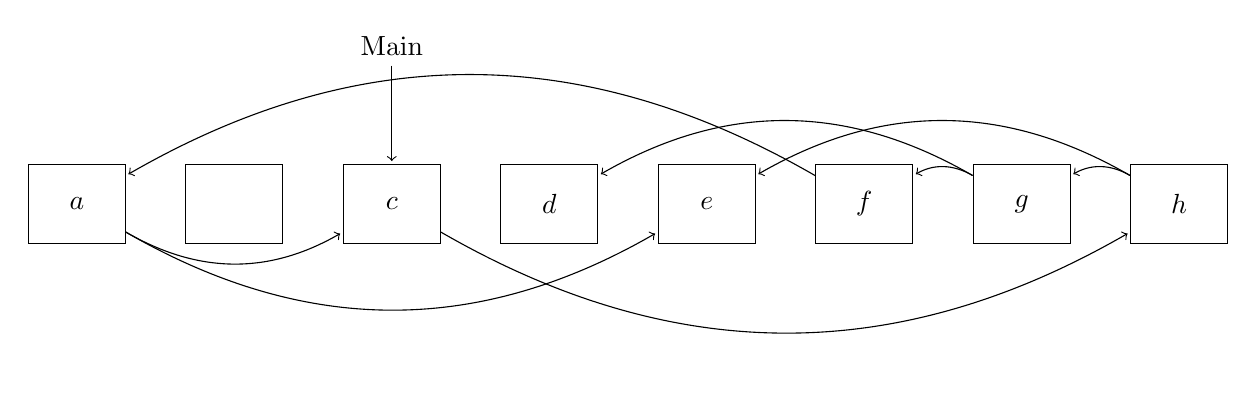
\begin{tikzpicture}[shorten >=1pt,node distance=2cm,on grid,auto]
    \tikzset{
      rect1/.style = {
        shape = rectangle,
        draw = black,
        text width = 1cm,
        align = center,
        minimum height = 1cm,
      }
    }
    \node[rect1] 			(a) 					{$a$};
    \node[rect1] 			(b) 	[right=of a]	{};
    \node[rect1]			(c) 	[right=of b] 	{$c$};
    \node[rect1] 			(d) 	[right=of c] 	{$d$};
    \node[rect1] 			(e) 	[right=of d] 	{$e$};
    \node[rect1] 			(f) 	[right=of e]	{$f$};
    \node[rect1] 			(g) 	[right=of f]	{$g$};
    \node[rect1] 			(h) 	[right=of g]	{$h$};
    \node (Main)[above = of c]{Main};
    \path[->]
    (a) 	edge	[bend right]		node 	{} 		(e)
        edge	[bend right] 	node 	{} 		(c)
    %(b)		edge	[bend right] 	node 	{} 		(d)
    (c)		edge	[bend right] 	node 	{} 		(h)
    (f) 	edge	[bend right] 	node 	{} 		(a)
    (g) 	edge	[bend right] 	node 	{} 		(d)
        edge	[bend right] 	node 	{} 		(f)
    (h) 	edge 	[bend right] 	node 	{} 		(e)
        edge 	[bend right] 	node 	{} 		(g)
        (Main) 	edge 	[] 	node 	{} 		(c)
     ;
  \end{tikzpicture}\end{center}
\item Copy Collector


\begin{center}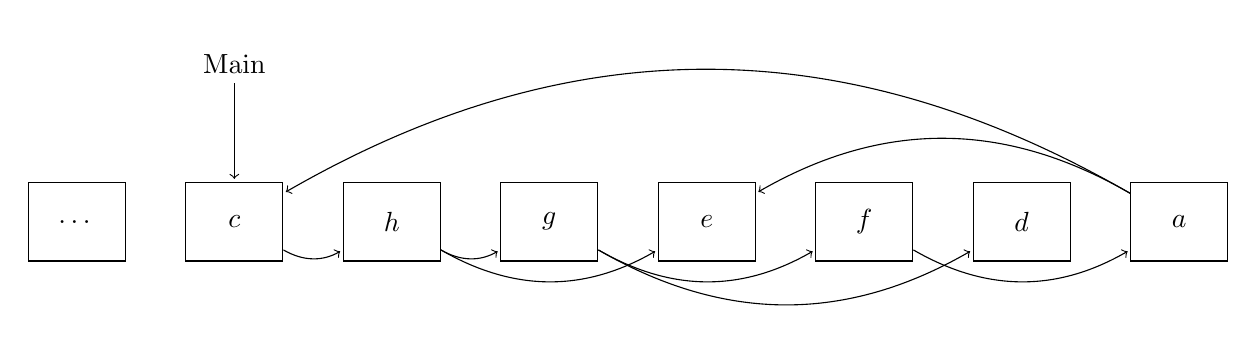
\begin{tikzpicture}[shorten >=1pt,node distance=2cm,on grid,auto]
  \tikzset{
    rect1/.style = {
      shape = rectangle,
      draw = black,
      text width = 1cm,
      align = center,
      minimum height = 1cm,
    }
  }
  \node[rect1]			(0) 	 	{$\dots$};
  \node[rect1]			(c) 	 [right=of 0]	{$c$};
  \node[rect1] 			(h) 	[right=of c]	{$h$};
  \node[rect1] 			(g) 	[right=of h]	{$g$};
  \node[rect1] 			(e) 	[right=of g] 	{$e$};
  \node[rect1] 			(f) 	[right=of e]	{$f$};
  \node[rect1] 			(d) 	[right=of f] 	{$d$};
  \node[rect1] 			(a) 	[right=of d]	{$a$};





  
  \node (Main)[above = of c]{Main};
  \path[->]
  (a) 	edge	[bend right]		node 	{} 		(e)
      edge	[bend right] 	node 	{} 		(c)
  %(b)		edge	[bend right] 	node 	{} 		(d)
  (c)		edge	[bend right] 	node 	{} 		(h)
  (f) 	edge	[bend right] 	node 	{} 		(a)
  (g) 	edge	[bend right] 	node 	{} 		(d)
      edge	[bend right] 	node 	{} 		(f)
  (h) 	edge 	[bend right] 	node 	{} 		(e)
      edge 	[bend right] 	node 	{} 		(g)
      (Main) 	edge 	[] 	node 	{} 		(c)
   ;
\end{tikzpicture}\end{center}

\item Reference Counting

\begin{center}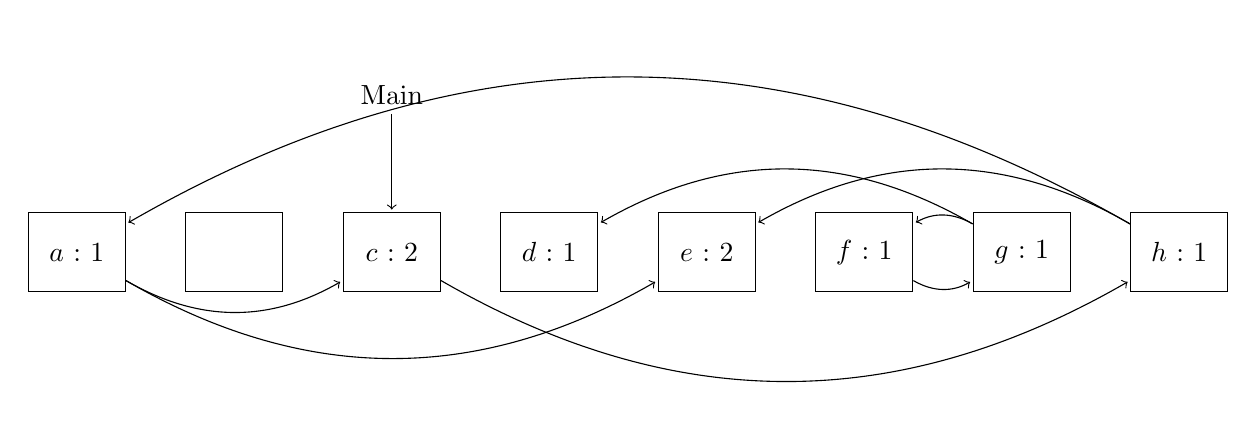
\begin{tikzpicture}[shorten >=1pt,node distance=2cm,on grid,auto]
  \tikzset{
    rect1/.style = {
      shape = rectangle,
      draw = black,
      text width = 1cm,
      align = center,
      minimum height = 1cm,
    }
  }
  \node[rect1] 			(a) 					{$a: 1$};
  \node[rect1] 			(b) 	[right=of a]	{};
  \node[rect1]			(c) 	[right=of b] 	{$c:2$};
  \node[rect1] 			(d) 	[right=of c] 	{$d:1$};
  \node[rect1] 			(e) 	[right=of d] 	{$e:2$};
  \node[rect1] 			(f) 	[right=of e]	{$f:1$};
  \node[rect1] 			(g) 	[right=of f]	{$g:1$};
  \node[rect1] 			(h) 	[right=of g]	{$h:1$};
  \node (Main)[above = of c]{Main};
  \path[->]
  (a) 	edge	[bend right]		node 	{} 		(e)
      edge	[bend right] 	node 	{} 		(c)
 % (b)		edge	[bend right] 	node 	{} 		(f)
  (c)		edge	[bend right] 	node 	{} 		(h)
  (f) 	edge	[bend right] 	node 	{} 		(g)
  (g) 	edge	[bend right] 	node 	{} 		(f)
      edge	[bend right] 	node 	{} 		(d)
  (h) 	edge 	[bend right] 	node 	{} 		(e)
      edge 	[bend right] 	node 	{} 		(a)
      (Main) 	edge 	[] 	node 	{} 		(c)
   ;
\end{tikzpicture}\end{center}
\end{enumerate}
  \item (10 pts) Suppose the cost $c_i$ is every reachable words' instruction number, comapare 3 algorithms, let $H$ be the size of the heap, let $R$ be the reachable word's data size, when will the Mark and Sweep outperform Copy Collector. 
  \newline
  The cost of Mark and Sweep: 
  \item (10 pts) Suppose the marking process is multithreaded, use the above example show that tricolor marking with write barrier is thread safe.


  \begin{center}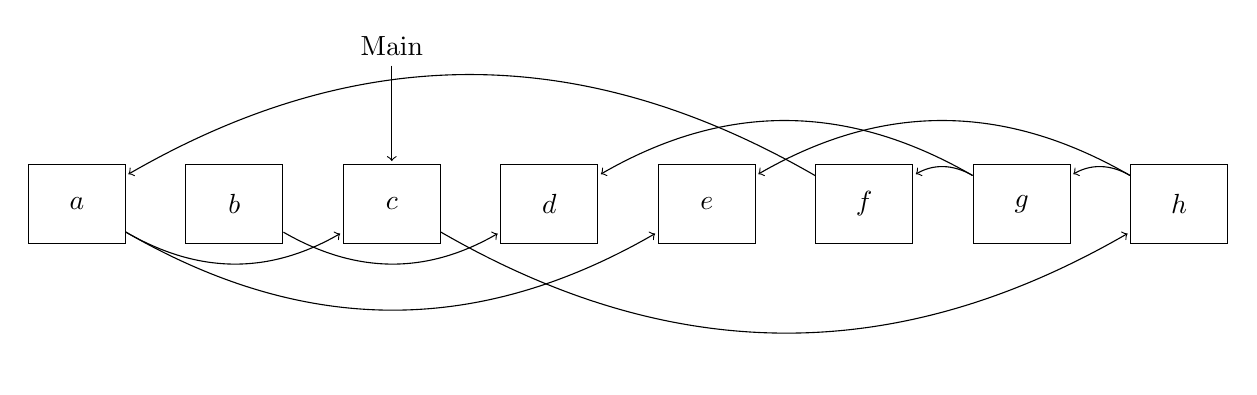
\begin{tikzpicture}[shorten >=1pt,node distance=2cm,on grid,auto]
    \tikzset{
      rect1/.style = {
        shape = rectangle,
        draw = black,
        text width = 1cm,
        align = center,
        minimum height = 1cm,
      }
    }
    \node[rect1] 			(a) 					{$a$};
    \node[rect1] 			(b) 	[right=of a]	{$b$};
    \node[rect1]			(c) 	[right=of b] 	{$c$};
    \node[rect1] 			(d) 	[right=of c] 	{$d$};
    \node[rect1] 			(e) 	[right=of d] 	{$e$};
    \node[rect1] 			(f) 	[right=of e]	{$f$};
    \node[rect1] 			(g) 	[right=of f]	{$g$};
    \node[rect1] 			(h) 	[right=of g]	{$h$};
    \node (Main)[above = of c]{Main};
    \path[->]
    (a) 	edge	[bend right]		node 	{} 		(e)
        edge	[bend right] 	node 	{} 		(c)
    (b)		edge	[bend right] 	node 	{} 		(d)
    (c)		edge	[bend right] 	node 	{} 		(h)
    (f) 	edge	[bend right] 	node 	{} 		(a)
    (g) 	edge	[bend right] 	node 	{} 		(d)
        edge	[bend right] 	node 	{} 		(f)
    (h) 	edge 	[bend right] 	node 	{} 		(e)
        edge 	[bend right] 	node 	{} 		(g)
        (Main) 	edge 	[] 	node 	{} 		(c)
     ;
  \end{tikzpicture}\end{center}


  \begin{center}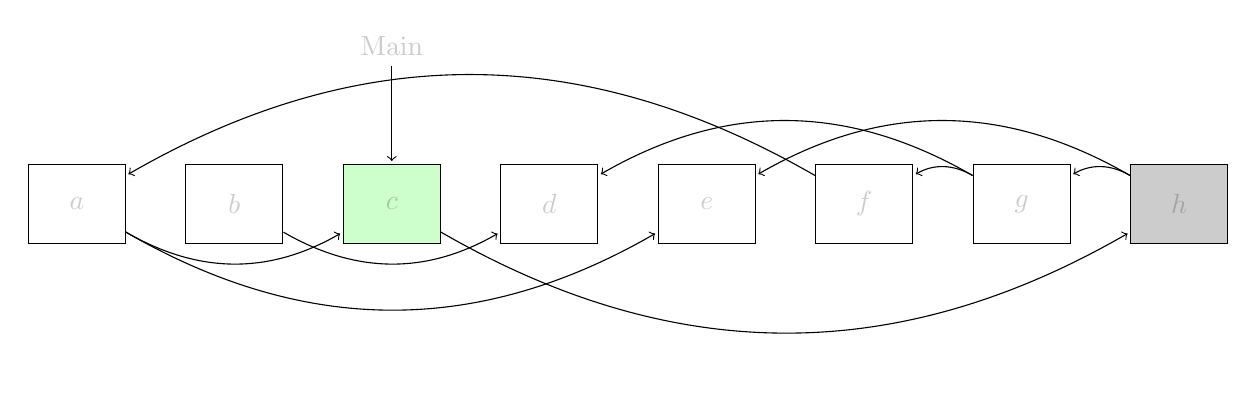
\begin{tikzpicture}[shorten >=1pt,node distance=2cm,on grid,auto, fill opacity=0.2]
    \tikzset{
      rect1/.style = {
        shape = rectangle,
        draw = black,
        text width = 1cm,
        align = center,
        minimum height = 1cm,
      }
    }
    \node[rect1] 			(a) 					{$a$};
    \node[rect1] 			(b) 	[right=of a]	{$b$};
    \node[rect1, fill=green]			(c) 	[right=of b] 	{$c$};
    \node[rect1] 			(d) 	[right=of c] 	{$d$};
    \node[rect1] 			(e) 	[right=of d] 	{$e$};
    \node[rect1] 			(f) 	[right=of e]	{$f$};
    \node[rect1] 			(g) 	[right=of f]	{$g$};
    \node[rect1, fill=black] 			(h) 	[right=of g]	{$h$};
    \node (Main)[above = of c]{Main};
    \path[->]
    (a) 	edge	[bend right]		node 	{} 		(e)
        edge	[bend right] 	node 	{} 		(c)
    (b)		edge	[bend right] 	node 	{} 		(d)
    (c)		edge	[bend right] 	node 	{} 		(h)
    (f) 	edge	[bend right] 	node 	{} 		(a)
    (g) 	edge	[bend right] 	node 	{} 		(d)
        edge	[bend right] 	node 	{} 		(f)
    (h) 	edge 	[bend right] 	node 	{} 		(e)
        edge 	[bend right] 	node 	{} 		(g)
        (Main) 	edge 	[] 	node 	{} 		(c)
     ;
  \end{tikzpicture}\end{center}

  \begin{center}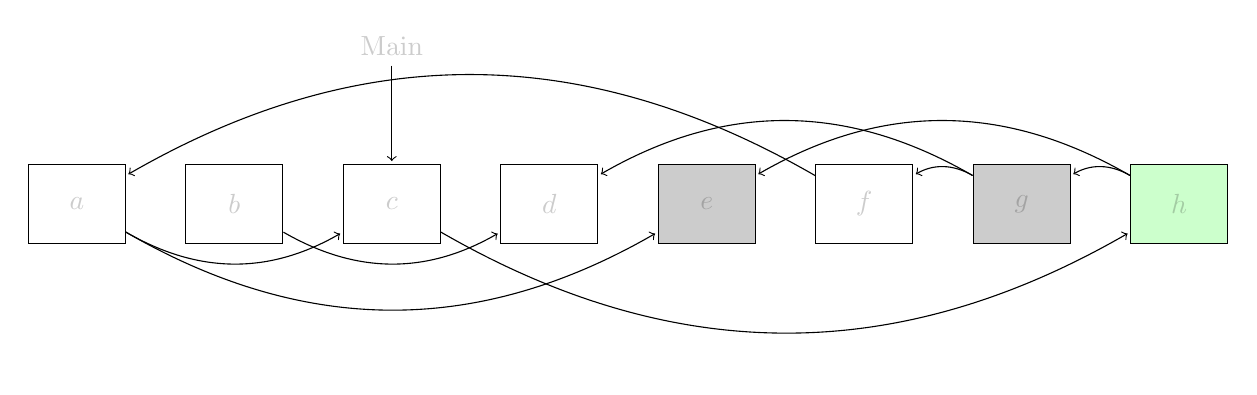
\begin{tikzpicture}[shorten >=1pt,node distance=2cm,on grid,auto, fill opacity=0.2]
    \tikzset{
      rect1/.style = {
        shape = rectangle,
        draw = black,
        text width = 1cm,
        align = center,
        minimum height = 1cm,
      }
    }
    \node[rect1] 			(a) 					{$a$};
    \node[rect1] 			(b) 	[right=of a]	{$b$};
    \node[rect1]			(c) 	[right=of b] 	{$c$};
    \node[rect1] 			(d) 	[right=of c] 	{$d$};
    \node[rect1,fill=black]		(e) 	[right=of d] 	{$e$};
    \node[rect1] 			(f) 	[right=of e]	{$f$};
    \node[rect1,fill=black] 			(g) 	[right=of f]	{$g$};
    \node[rect1,  fill=green] 			(h) 	[right=of g]	{$h$};
    \node (Main)[above = of c]{Main};
    \path[->]
    (a) 	edge	[bend right]		node 	{} 		(e)
        edge	[bend right] 	node 	{} 		(c)
    (b)		edge	[bend right] 	node 	{} 		(d)
    (c)		edge	[bend right] 	node 	{} 		(h)
    (f) 	edge	[bend right] 	node 	{} 		(a)
    (g) 	edge	[bend right] 	node 	{} 		(d)
        edge	[bend right] 	node 	{} 		(f)
    (h) 	edge 	[bend right] 	node 	{} 		(e)
        edge 	[bend right] 	node 	{} 		(g)
        (Main) 	edge 	[] 	node 	{} 		(c)
     ;
  \end{tikzpicture}\end{center}

  \begin{center}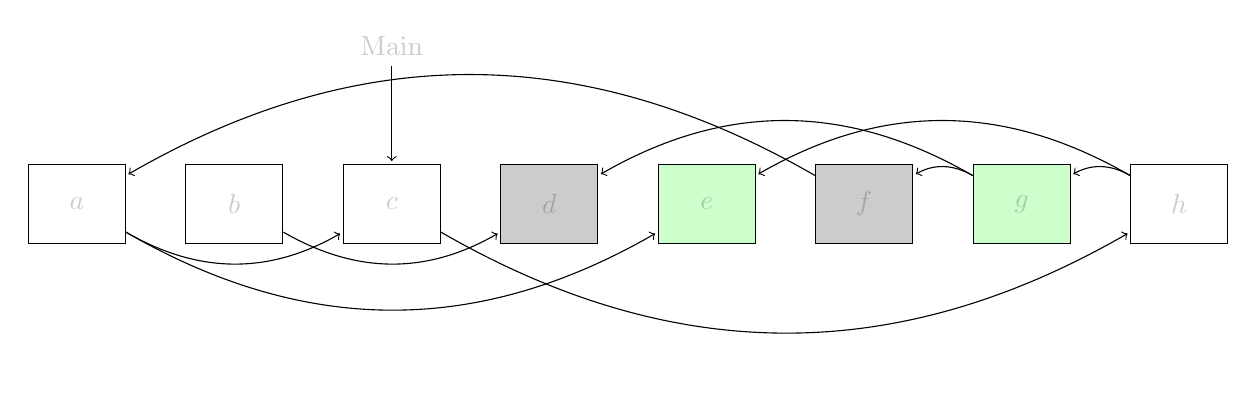
\begin{tikzpicture}[shorten >=1pt,node distance=2cm,on grid,auto, fill opacity=0.2]
    \tikzset{
      rect1/.style = {
        shape = rectangle,
        draw = black,
        text width = 1cm,
        align = center,
        minimum height = 1cm,
      }
    }
    \node[rect1] 			(a) 					{$a$};
    \node[rect1] 			(b) 	[right=of a]	{$b$};
    \node[rect1]			(c) 	[right=of b] 	{$c$};
    \node[rect1,  fill=black]	(d) 	[right=of c] 	{$d$};
    \node[rect1, fill=green]		(e) 	[right=of d] 	{$e$};
    \node[rect1,  fill=black] 			(f) 	[right=of e]	{$f$};
    \node[rect1, fill=green] 			(g) 	[right=of f]	{$g$};
    \node[rect1 ] 			(h) 	[right=of g]	{$h$};
    \node (Main)[above = of c]{Main};
    \path[->]
    (a) 	edge	[bend right]		node 	{} 		(e)
        edge	[bend right] 	node 	{} 		(c)
    (b)		edge	[bend right] 	node 	{} 		(d)
    (c)		edge	[bend right] 	node 	{} 		(h)
    (f) 	edge	[bend right] 	node 	{} 		(a)
    (g) 	edge	[bend right] 	node 	{} 		(d)
        edge	[bend right] 	node 	{} 		(f)
    (h) 	edge 	[bend right] 	node 	{} 		(e)
        edge 	[bend right] 	node 	{} 		(g)
        (Main) 	edge 	[] 	node 	{} 		(c)
     ;
  \end{tikzpicture}\end{center}
\end{enumerate}

\begin{center}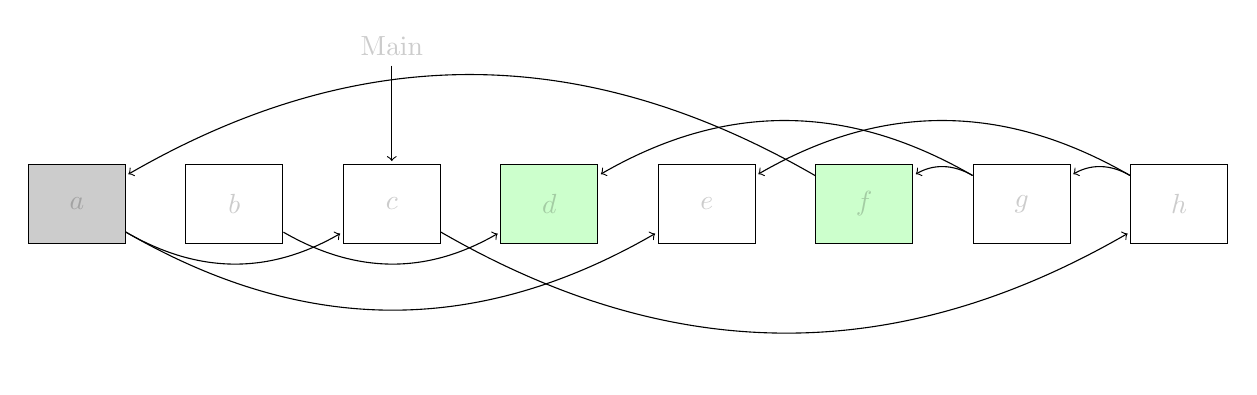
\begin{tikzpicture}[shorten >=1pt,node distance=2cm,on grid,auto, fill opacity=0.2]
  \tikzset{
    rect1/.style = {
      shape = rectangle,
      draw = black,
      text width = 1cm,
      align = center,
      minimum height = 1cm,
    }
  }
  \node[rect1,  fill=black] 			(a) 					{$a$};
  \node[rect1] 			(b) 	[right=of a]	{$b$};
  \node[rect1]			(c) 	[right=of b] 	{$c$};
  \node[rect1,  fill=green]	(d) 	[right=of c] 	{$d$};
  \node[rect1]		(e) 	[right=of d] 	{$e$};
  \node[rect1,  fill=green] 			(f) 	[right=of e]	{$f$};
  \node[rect1] 			(g) 	[right=of f]	{$g$};
  \node[rect1 ] 			(h) 	[right=of g]	{$h$};
  \node (Main)[above = of c]{Main};
  \path[->]
  (a) 	edge	[bend right]		node 	{} 		(e)
      edge	[bend right] 	node 	{} 		(c)
  (b)		edge	[bend right] 	node 	{} 		(d)
  (c)		edge	[bend right] 	node 	{} 		(h)
  (f) 	edge	[bend right] 	node 	{} 		(a)
  (g) 	edge	[bend right] 	node 	{} 		(d)
      edge	[bend right] 	node 	{} 		(f)
  (h) 	edge 	[bend right] 	node 	{} 		(e)
      edge 	[bend right] 	node 	{} 		(g)
      (Main) 	edge 	[] 	node 	{} 		(c)
   ;
\end{tikzpicture}\end{center}


\end{enumerate}
\end{document}

